\chapter{Šroubovice}
Nyní se budeme věnovat prostorovým křivkám. Nejčastěji se v praxi používá šroubovice na válcové ploše. \\
Abychom mohli popsat šroubovici bodu, musíme zadat \textit{šroubový pohyb}. \\[5pt]
\textbf{Šroubový pohyb} je dán
\begin{enumerate}
	\item osou \textit{o},
	\item smyslem (pravotočivý a levotočivý),
	\item výškou závitu v.
\end{enumerate}
Osa šroubového pohybu může být libovolná přímka v prostoru, pro zjednodušení budeme v dalším textu používat osu \textit{z}
souřadné soustavy $(O, x, y, z)$. Používáme vždy \textit{pravotočivou} kartézskou souřadnou soustavu, kterou využívají i grafické
programy. \\
Šroubový pohyb je složením rovnoměrného rotačního pohybu a rovnoměrného translačního pohybu. \\
Pokud je rotační pohyb proti směru hodinových ručiček a translační pohyb ve směru kladné poloosy osy \textit{z} nebo rotační pohyb
ve směru hodinových ručiček a translační pohyb ve směru záporné poloosy osy \textit{z}, je šroubový pohyb pravotočivý, v opačném
případě je levotočivý.
\begin{figure}[H]
	\centering
	\begin{subfigure}[b]{0.4\textwidth}
		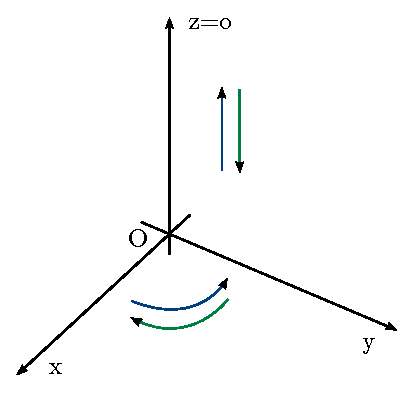
\includegraphics[width=\textwidth]{sroubovice-teorie1.eps}
		\caption{Pravotočivý šroubový pohyb}
	\end{subfigure}%
	\quad
	\begin{subfigure}[b]{0.4\textwidth}
		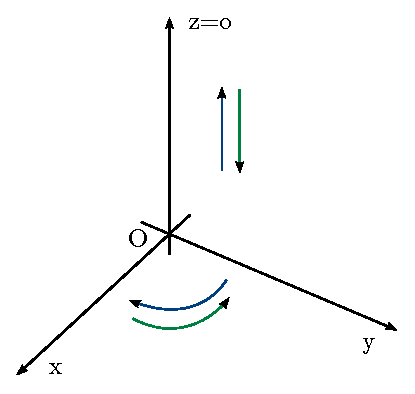
\includegraphics[width=\textwidth]{sroubovice-teorie2.eps}
		\caption{Levotočivý šroubový pohyb}
	\end{subfigure}%
\end{figure}
\clearpage
\noindent Vyberme si bod \textit{A} v prostoru, který neleží na ose šroubového
pohybu. Bod se při šroubovém pohybu rovnoměrně otáčí kolem osy \textit{o} a zároveň se rovnoměrně posunuje ve směru osy \textit{o}.
Šroubovice bodu \textit{A} leží na válcové ploše, jejíž osou je osa \textit{o} šroubového pohybu a poloměr je roven vzdáleností bodu \textit{A} od osy \textit{o}. \\
Výška závitu \textit{v} je vzdálenost bodu $A$ a bodu $A'$, kde $A$ a $A'$ jsou body na povrchové přímce \textit{p} válcové plochy
a mezi nimi není žádný jiný bod šroubovice. Část šroubovice mezi body $A$ a $A'$ je tzv. 1 závit šroubovice a odpovídá otočení o
úhel $2\pi$.
\begin{figure}[H]
	\centering
	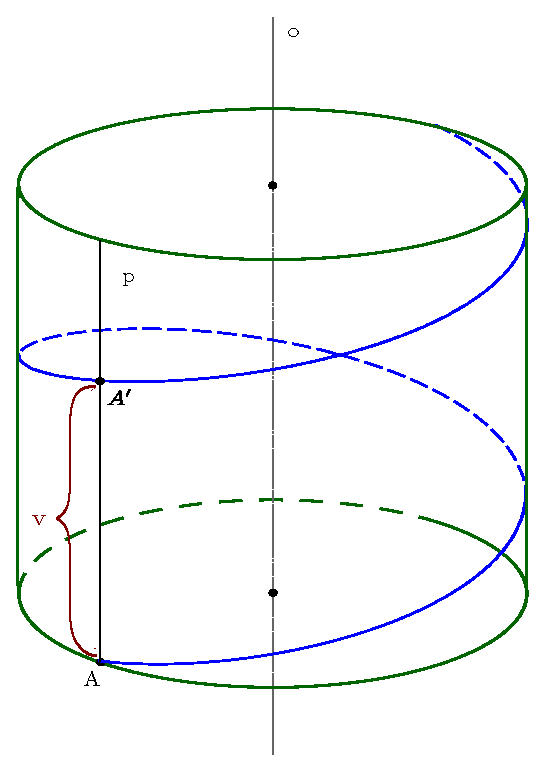
\includegraphics[width=0.3\textwidth]{sroubovice-teorie3.eps}
	\caption{Šroubovice na válcové ploše}
\end{figure}
\noindent{}Po rozstřižení válcové plochy podél \textit{p} a rozvinutí do roviny máme následující obrázek.
\begin{figure}[H]
	\centering
	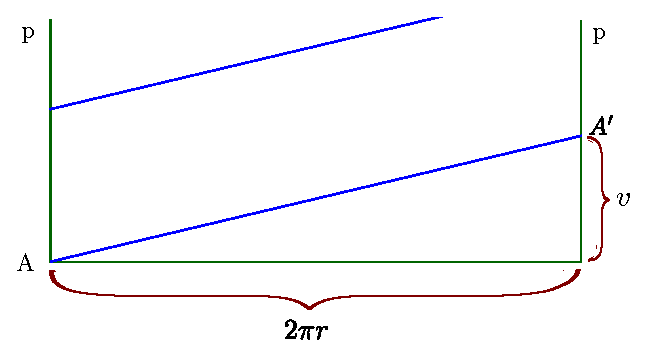
\includegraphics[width=0.8\textwidth]{sroubovice-teorie4.eps}
	\caption{Válcová plocha rozstřižená podél přímky \textit{p} a rozvinutá do roviny}
\end{figure}
\noindent{}To je také návodem, jak si snadno šroubovici \uv{vyrobit}. Stačí slepit papír, na kterém jsme narýsovali úsečku pro jeden závit nebo více
rovnoběžných úseček pro více závitů. \\
V technické praxi se často užívá místo výšky závitu tzv. \textit{redukovaná výška závitu}, kterou značíme $v_0$. Je to výška posunutí
odpovídající otočení o úhel 1 radián (přibližně $57^{\circ}17'45''$). Úhlu 1 radián odpovídá délka oblouku kružnice rovná poloměru \textit{r} kružnice. \\
Z obrázku
\begin{figure}[H]
	\centering
	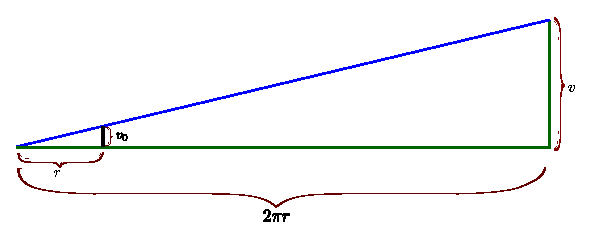
\includegraphics[width=0.8\textwidth]{sroubovice-teorie5.eps}
	\caption{Ilustrační obrázek}
\end{figure}
\noindent snadno odvodíme vztah mezi výškou \textit{v} závitu a redukovanou výškou $v_0$:
\begin{align*}
	\frac{v_0}{r} & = \frac{v}{2 \pi r} \\
	v_0           & = \frac{v}{2\pi}    
\end{align*}
Jak napsat parametrické vyjádření šroubovice bodu $A=[a_1, a_2, a_3]$? \\
Zadejme šroubový pohyb:
\begin{enumerate}
	\item osa \textit{o} je souřadnicová osa \textit{z},
	\item pravotočivý (resp. levotočivý),
	\item výškou závitu je \textit{v} (nebo redukovaná výška je $v_0$).
\end{enumerate}
Šroubovice leží na válcové ploše, jejíž osou je osa \textit{z}. Průnik této plochy s půdorysnou $(x, y)$ je kružnice.
Začneme parametrickým popisem kružnice v rovině $(x, y)$, střed kružnice je bod $[0,0]$ a kružnice prochází bodem $[a_1, a_2]$. \\
Je-li šroubový pohyb \emph{pravotočivý}, musíme kružnici popsat tak, aby byla probíhána \emph{proti} směru hodinových ručiček, tj. v kladném směru.
Navíc požadujeme, aby pro $t=0$ byl výchozí bod $[a_1, a_2]$. \\
Je-li šroubový pohyb levotočivý, musíme kružnici popsat tak, aby byla probíhána ve směru hodinových ručiček, tj. v záporném směru. Opět v čase $t=0$
jsme v bodě $[a_1, a_2]$. Tedy
\begin{align*}
	m(t) & = [a_1\cos{t}-a_2\sin{t}, a_2\cos{t}+a_1\sin{t}] \text{ pro kladný směr},   \\
	m(t) & = [a_1\cos{t}+a_2\sin{t}, a_2\cos{t}-a_1\sin{t}] \text{ pro záporný směr}. 
\end{align*}
Třetí \textit{z}-ová souřadnice se týká posunutí, parametrický popis pravotočivé šroubovice je
$$k(t) = [a_1\cos{t}-a_2\sin{t}, a_2\cos{t}+a_1\sin{t}, a_3+v_0 t], t \in \mathbb{R}.$$
Parametrický popis levotočivé šroubovice je
$$k(t) = [a_1\cos{t}+a_2\sin{t}, a_2\cos{t}-a_1\sin{t}, a_3+v_0 t], t \in \mathbb{R}.$$
Šroubovice je neomezená křivka v obou směrech. \\
Důležitý je jeden závit šroubovice, který se dále jen posunuje. Pokud chceme popsat 1 závit, bereme parametr \textit{t} z intervalu délky $2\pi$.
Použijeme-li výše uvedený parametrický popis, je $k(0)=A$ a pro jeden závit s krajním bodem \textit{A} bereme $t\in\langle0, 2\pi\rangle$.
\clearpage
\subsection*{Příklad 1}
Napište parametrické vyjádření šroubovice bodu $A=[0,4,0]$. Osa šroubového pohybu je osa \textit{z}, šroubový pohyb je
\begin{enumerate}
	\item pravotočivý
	\item levotočivý
\end{enumerate}
Výška závitu $v=12$. \\[10pt]
\textbf{Řešení: } \\
\begin{enumerate}
	\item Popíšeme kružnici \textit{m} v rovině $(x,y)$, střed je bod $[0,0]$, výchozí bod je bod $[x_A, y_A]=[0,4]$, kružnice je probíhána v kladném směru:
	      $$m(t) = \left[-4\sin{t}, 4\cos{t}\right].$$
	      Pro popis pravotočivé šroubovice doplníme \textit{z}-ovou souřadnici $z_A+v_0t$, kde $v_0=\frac{v}{2\pi}=\frac{12}{2\pi}=\frac{6}{\pi}$:
	      $$k(t) = \left[-4\sin{t}, 4\cos{t}, \frac{6}{\pi}t\right], t \in \mathbb{R},$$
	      (nebo $t \in \langle0, 2\pi\rangle$ pro 1 závit šroubovice).
	\item Parametrický popis levotočivé šroubovice získáme z předchozího popisu změnou znaménka u funkce $\sin$ (oběh kružnice v záporném směru):
	      $$k(t) = \left[4\sin{t}, 4\cos{t}, \frac{6}{\pi}t\right], t \in \mathbb{R},$$
	      (nebo $t \in \langle0, 2\pi\rangle$ pro 1 závit). 	
	      \clearpage
	      \begin{figure}[H]
	      	\centering
	      	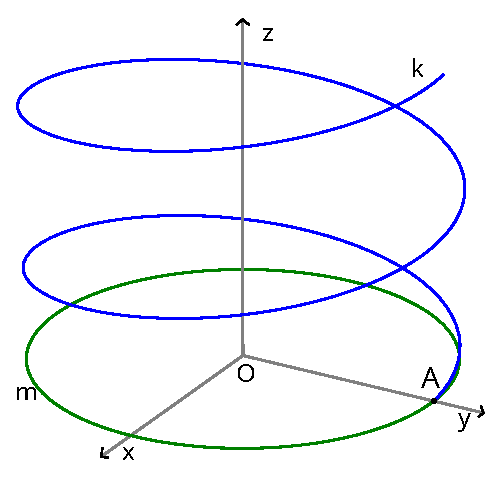
\includegraphics[width=0.5\textwidth]{sroubovice1.eps}
	      	\caption{Pravotočivá šroubovice pro $t \in \langle0, 4\pi\rangle$}
	      \end{figure}	
	      \begin{figure}[H]
	      	\centering
	      	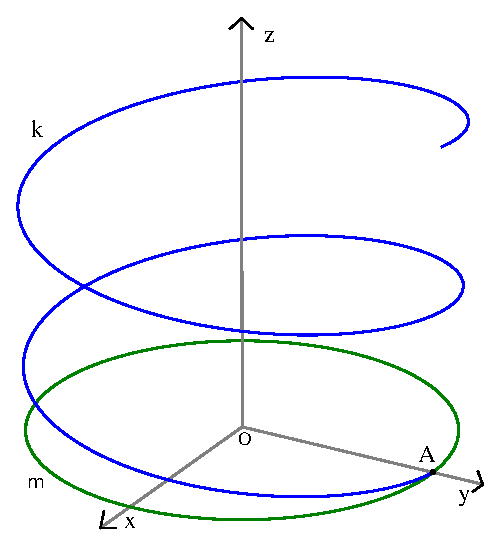
\includegraphics[width=0.5\textwidth]{sroubovice2.eps}
	      	\caption{Levotočivá šroubovice pro $t \in \langle0, 4\pi\rangle$}
	      	
	      \end{figure}	 	
\end{enumerate}
\clearpage
\subsection*{Příklad 2}
Napište parametrické vyjádření šroubovice bodu $A=[-4,0,0]$. Osa šroubového pohybu je osa \textit{z},
šroubový pohyb je
\begin{enumerate}
	\item pravotočivý
	\item levotočivý
\end{enumerate}
Výška závitu je $v=18$. \\[10pt]
\textbf{Řešení: } 
\begin{enumerate}
	\item Popíšeme kružnici v rovině $(x,y)$, střed je bod $[0,0]$, výchozí bod je bod $[x_A, y_A]=[-4,0]$, kružnice je probíhána v kladném směru:
	      $$m(t) = \left[-4\cos{t}, -4\sin{t}\right].$$
	      Pro popis pravotočivé šroubovice doplníme \textit{z}-ovou souřadnici $z_A+v_0t$, kde $v_0=\frac{v}{2\pi}=\frac{18}{2\pi}=\frac{9}{\pi}$:
	      $$k(t) = \left[-4\cos{t}, -4\sin{t}, \frac{9}{\pi}t\right], t \in \mathbb{R},$$
	      (nebo $t \in \langle0, 2\pi\rangle$ pro 1 závit šroubovice).
	      \begin{figure}[H]
	      	\centering
	      	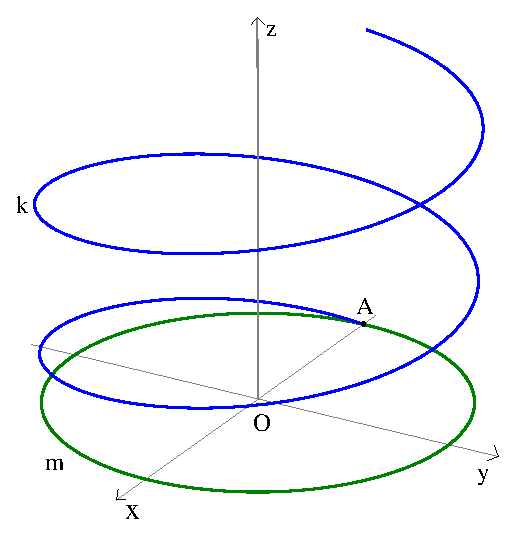
\includegraphics[width=0.5\textwidth]{sroubovice3.eps}
	      	\caption{Pravotočivá šroubovice pro $t \in \langle0, 4\pi\rangle$}
	      	
	      \end{figure}	 	
	\item Parametrický popis levotočivé šroubovice získáme z předchozího popisu změnou znaménka u funkce $\sin$ (oběh kružnice v záporném směru):
	      $$k(t) = \left[-4\cos{t}, 4\sin{t}, \frac{9}{\pi}t\right], t \in \mathbb{R},$$
	      (nebo $t \in \langle0, 2\pi\rangle$ pro 1 závit). 	
	      \begin{figure}[H]
	      	\centering
	      	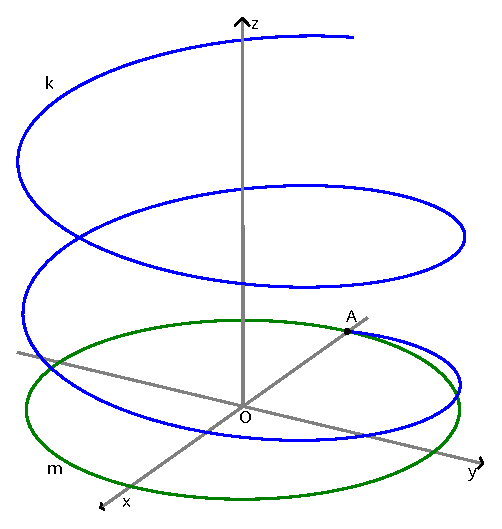
\includegraphics[width=0.5\textwidth]{sroubovice4.eps}
	      	\caption{Levotočivá šroubovice pro $t \in \langle0, 4\pi\rangle$}
	      	
	      \end{figure}	 	
\end{enumerate}
\clearpage
\subsection*{Příklad 3}
Napište parametrické vyjádření šroubovice bodu $A=[0,-4,0]$. Osa šroubového pohybu je osa \textit{z},
šroubový pohyb je
\begin{enumerate}
	\item pravotočivý
	\item levotočivý
\end{enumerate}
Redukovaná výška závitu je $v_0=3$. \\[10pt]
\textbf{Řešení: } 
\begin{enumerate}
	\item Popíšeme kružnici v rovině $(x,y)$, střed je bod $[0,0]$, výchozí bod je bod $[x_A, y_A]=[0,-4]$, kružnice je probíhána v kladném směru:
	      $$m(t) = \left[4\sin{t}, -4\cos{t}\right].$$
	      Pro popis pravotočivé šroubovice doplníme \textit{z}-ovou souřadnici $z_A+v_0t$:
	      $$k(t) = \left[4\sin{t}, -4\cos{t}, 3t\right], t \in \mathbb{R},$$
	      (nebo $t \in \langle0, 2\pi\rangle$ pro 1 závit šroubovice).
	      \begin{figure}[H]
	      	\centering
	      	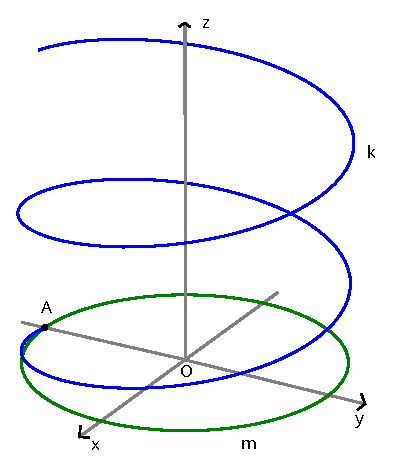
\includegraphics[width=0.5\textwidth]{sroubovice5.eps}
	      	\caption{Pravotočivá šroubovice pro $t \in \langle0, 4\pi\rangle$}
	      	
	      \end{figure}	 	
	      \clearpage
	\item Parametrický popis levotočivé šroubovice získáme z předchozího popisu změnou znaménka u funkce $\sin$ (oběh kružnice v záporném směru):
	      $$k(t) = \left[-4\sin{t}, -4\cos{t}, 3t\right], t \in \mathbb{R},$$
	      (nebo $t \in \langle0, 2\pi\rangle$ pro 1 závit). 	
	      \begin{figure}[H]
	      	\centering
	      	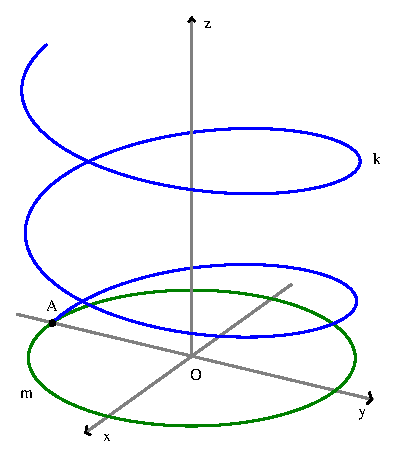
\includegraphics[width=0.5\textwidth]{sroubovice6.eps}
	      	\caption{Levotočivá šroubovice pro $t \in \langle0, 4\pi\rangle$}
	      	
	      \end{figure}	 	
\end{enumerate}
\clearpage
\subsection*{Příklad 4}
Napište parametrické vyjádření šroubovice bodu $A=[4,0,3]$. Osa šroubového pohybu je osa \textit{z},
šroubový pohyb je
\begin{enumerate}
	\item pravotočivý
	\item levotočivý
\end{enumerate}
Redukovaná výška závitu je $v_0=2$. \\
Dále popište tečnu šroubovice v bodě \textit{A}. \\[10pt]
\textbf{Řešení: } 
\begin{enumerate}
	\item Popíšeme kružnici v rovině $(x,y)$, střed je bod $[0,0]$, výchozí bod je bod $[x_A, y_A]=[4,0]$, kružnice je probíhána v kladném směru:
	      $$m(t) = \left[4\cos{t}, 4\sin{t}\right].$$
	      Pro popis pravotočivé šroubovice doplníme \textit{z}-ovou souřadnici $z_A+v_0t$:
	      $$k(t) = \left[4\cos{t}, 4\sin{t}, 2t+3\right], t \in \mathbb{R},$$
	      (nebo $t \in \langle0, 2\pi\rangle$ pro 1 závit šroubovice). \\
	      Tečné vektory získáme derivováním
	      $$k'(t)=(-4\sin{t}, 4\cos{t}, 2).$$
	      Pro bod $A=k(0)$ je tečný vektor
	      $$k'(0)=(0,4,2)$$
	      a parametrický popis tečny \textit{p} je
	      $$p(s)=[4,4s,3+2s], s \in \mathbb{R}.$$
	\item Parametrický popis levotočivé šroubovice získáme z předchozího popisu změnou znaménka u funkce $\sin$ (oběh kružnice v záporném směru):
	      $$k(t) = \left[4\cos{t}, -4\sin{t}, 2t+3\right], t \in \mathbb{R},$$
	      (nebo $t \in \langle0, 2\pi\rangle$ pro 1 závit). 	\\
	      Tečné vektory získáme derivováním
	      $$k'(t)=(-4\sin{t}, -4\cos{t}, 2).$$
	      Pro bod $A=k(0)$ je tečný vektor
	      $$k'(0)=(0,-4,2)$$
	      a parametrický popis tečny \textit{p} je
	      $$p(s)=[4,-4s,3+2s], s \in \mathbb{R}.$$
	      \begin{figure}[H]
	      	\centering
	      	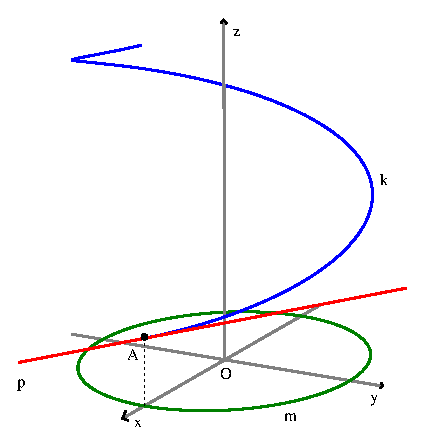
\includegraphics[width=0.5\textwidth]{sroubovice7.eps}
	      	\caption{Pravotočivá šroubovice pro $t \in \langle0, 2\pi\rangle$}
	      \end{figure}	 	
	      \begin{figure}[H]
	      	\centering
	      	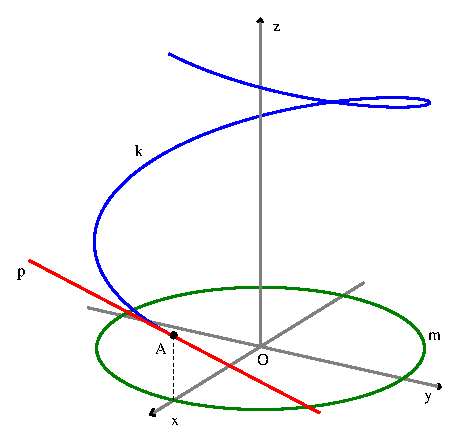
\includegraphics[width=0.5\textwidth]{sroubovice8.eps}
	      	\caption{Levotočivá šroubovice pro $t \in \langle0, 2\pi\rangle$}
	      	
	      \end{figure}	 	
\end{enumerate}
\clearpage

\subsection*{Příklad 5}
Napište parametrické vyjádření šroubovice bodu $A=[3,4,2]$. Osa pravotočivého šroubového pohybu je osa \textit{z},
výška závitu je $v=20$. \\
Dále popište tečny šroubovice v bodech \textit{A}, $k\left(\frac{\pi}{2}\right)$, $k(\pi)$ a $k(2\pi)$.\\[10pt]
\textbf{Řešení: } 
Popíšeme kružnici v rovině $(x,y)$, střed je bod $[0,0]$, výchozí bod je bod $[x_A, y_A]=[3,4]$, kružnice je probíhána v kladném směru:
$$m(t) = \left[3\cos{t}-4\sin{t}, 4\cos{t}+3\sin{t}\right].$$
Pro popis pravotočivé šroubovice doplníme \textit{z}-ovou souřadnici $z_A+v_0t$, kde $v_0=\frac{v}{2\pi}=\frac{20}{2\pi}=\frac{10}{\pi}$:
$$k(t) = \left[3\cos{t}-4\sin{t}, 4\cos{t}+3\sin{t}, \frac{10}{\pi}t+2\right], t \in \mathbb{R},$$
(nebo $t \in \langle0, 2\pi\rangle$ pro 1 závit šroubovice). \\
Tečné vektory získáme derivováním
$$k'(t)=\left(-3\sin{t}-4\cos{t}, 3\cos{t}-4\sin{t}, \frac{10}{\pi}\right).$$
Konkrétní tečné vektory jsou tedy:
\begin{align*}
	k'(0)                        & =\left(-4,3,\frac{10}{\pi}\right),   \\
	k'\left(\frac{\pi}{2}\right) & = \left(-3,-4,\frac{10}{\pi}\right), \\
	k'(\pi)                      & = \left(4,-3,\frac{10}{\pi}\right),  \\
	k'(2\pi)                     & = \left(-4,3,\frac{10}{\pi}\right).  
\end{align*}
V bodech:
\begin{align*}
	k(0)                        & =A=\left[3,4,2\right],   \\
	k\left(\frac{\pi}{2}\right) & = \left[-4,3,7\right],   \\
	k(\pi)                      & = \left[-3,-4,12\right], \\
	k(2\pi)                     & = \left[3,4,22\right]    
\end{align*} 	
je parametrický popis tečen:
\begin{align*}
	p_1(s) & = \left[3-4s,4+3s,2+\frac{10}{\pi}s\right], s \in \mathbb{R},    \\
	p_2(s) & = \left[-4-3s,3-4s,7+\frac{10}{\pi}s\right], s \in \mathbb{R},   \\
	p_3(s) & = \left[-3+4s,-4-3s,12+\frac{10}{\pi}s\right], s \in \mathbb{R}, \\
	p_4(s) & = \left[3-4s,4+3s,22+\frac{10}{\pi}s\right], s \in \mathbb{R}.   
\end{align*} 	
\begin{figure}[H]
	\centering
	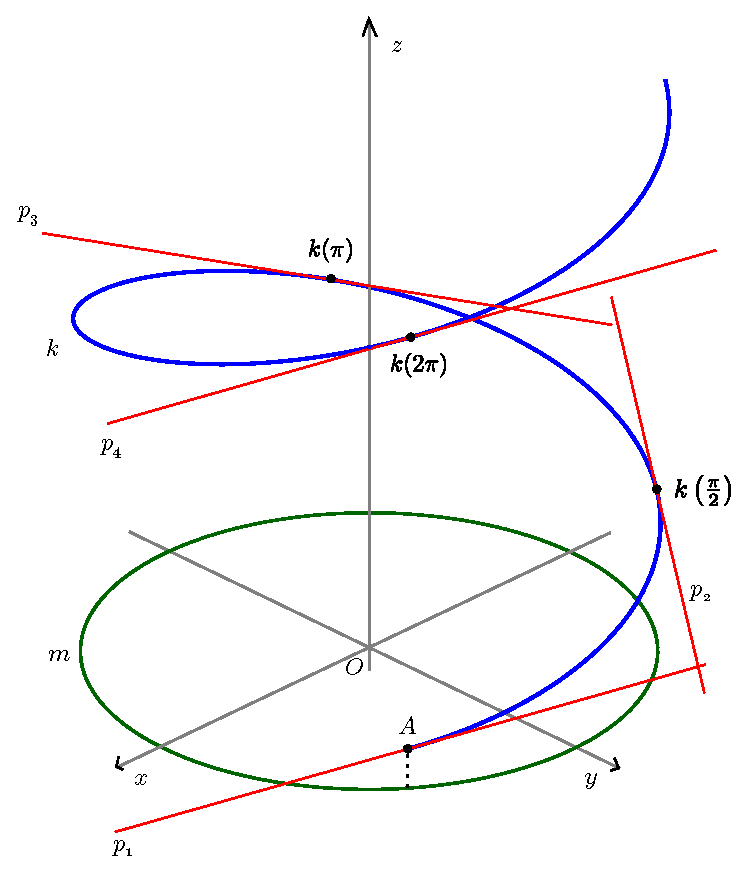
\includegraphics[width=0.7\textwidth]{sroubovice9-oprava.eps}
	\caption{Pravotočivá šroubovice pro $t \in \langle0, \frac{5\pi}{2}\rangle$}
	
\end{figure}	 	